%%%%%%%%%%%%%%%%%
%  Boson Tagger 
%%%%%%%%%%%%%%%%%
%\subsubsection{Boson Tagger}
\label{subsec:bkg_uncer_vtagger}

For the uncertainties associated with the boson tagger's background efficiency, we consider both the large-\(R\) jet-related uncertainties and the modelling uncertainties from multi-jet and $\gamma$+jets. 
The modelling uncertainties are estimated by comparing the nominal Pythia 8 and Sherpa samples against alternative Sherpa and Pythia 8 samples for multi-jet and $\gamma$+jets, respectively.
For more on how the tagger is defined, see \cite{ATL-PHYS-PUB-2020-017}.

Systematic uncertainties associated with the scale factors, which assess the boson tagger's relative performance in data versus MC, are thoroughly evaluated. 
These uncertainties encompass various aspects. For background uncertainties, factors such as matrix element variations, hadronization, radiation effects, and the impact of dijets or $\gamma$+jets events are considered. Signal uncertainties include considerations like the extrapolation at high-\(\pT\).

Further details on these recommendations are available on the central CP twiki \cite{JSSrecommendationSF}. Plots illustrating the impact of uncertainties on the Data/MC ratio for the \olep channel are presented in Figure \ref{fig:1LepVTaggerUnc}.

%%%
%%%For the boson tagger uncertainties related to the background efficiency measurement, the large-R jet related uncertainties as well as multi-jet and $\gamma$+jets modelling uncertainties are considered. 
%%%The modelling uncertainties are estimated from the nominal Pythia 8 and Sherpa sample in comparison to the alternative  Sherpa and Pythia 8 samples for multijet and $\gamma$+jets respectively. 
%%%For more on how the tagger is defined, see \cite{ATL-PHYS-PUB-2020-017}.
%%%
%%%Systematic uncertainties related to the scale factors used to quantify the relative performance 
%%%of the boson tagger in data versus MC are also considered; 
%%%detailed information are provided in the main recommendation twiki from the CP group \cite{JSSrecommendationSF}.
%%%
%%%In Figure \ref{fig:2lep_bkgUnc_BT} Data/MC ratios are plotted as a function of the mass of the tagging jets 
%%%for the different merged analysis regions of the 2-lepton channel and for the different boson tagger related uncertainties. 
%%%They are related to both background uncertainties, like matrix element, hadronisation, radiation effects,
%%%impact of dijets or $\gamma$+jets events, both to signal uncertainties, like extrapolation at high-\pT or
%%%extrapolation to the Z boson. Further details can be found on the central CP twiki for the recommendations
%%%\cite{JSSrecommendationSF}.
%%%The largest systematic uncertainty is related to the $\gamma$+jets modelling and is seen in the HP signal region. 
%%%In the merged CR the major systematic source is related to the efficiency uncertainty of the 80\% tagger working point 
%%%while in the LP SR major systematic sources (still less than 5\%) are related to the $\gamma$+jets modelling 
%%%and the efficiency uncertainty of the 50\% tagger working point. 
%%%The fact that the efficiency uncertainty of the 50\% tagger working point is relevant in the LP SR is not surprising 
%%%given the SF calculation in this region, which is defined as: 
%%%
%%%    \begin{equation}
%%%        SF_{LP} = \frac{\epsilon_{loose}SF_{eff,loose}- \epsilon_{tight}SF_{eff,tight} }{ \epsilon_{loose}- \epsilon_{tight}}
%%%    \end{equation}        
%%%.
%%%
%%%Similar plots showing the impact of the effect of the uncertainties around the Data/MC ratio 
%%%for the \olep channel are shown in Figure \ref{fig:1LepVTaggerUnc};
%%%the impact of all the SF related uncertainties on the MC shapes of the signal and bkg samples
%%%in the \zlep channel are shown in Figure \ref{fig:0LepVTaggerUnc}.

\begin{figure}[ht]
    \centering
    \begin{subfigure}[b]{0.3\textwidth}
        \centering
        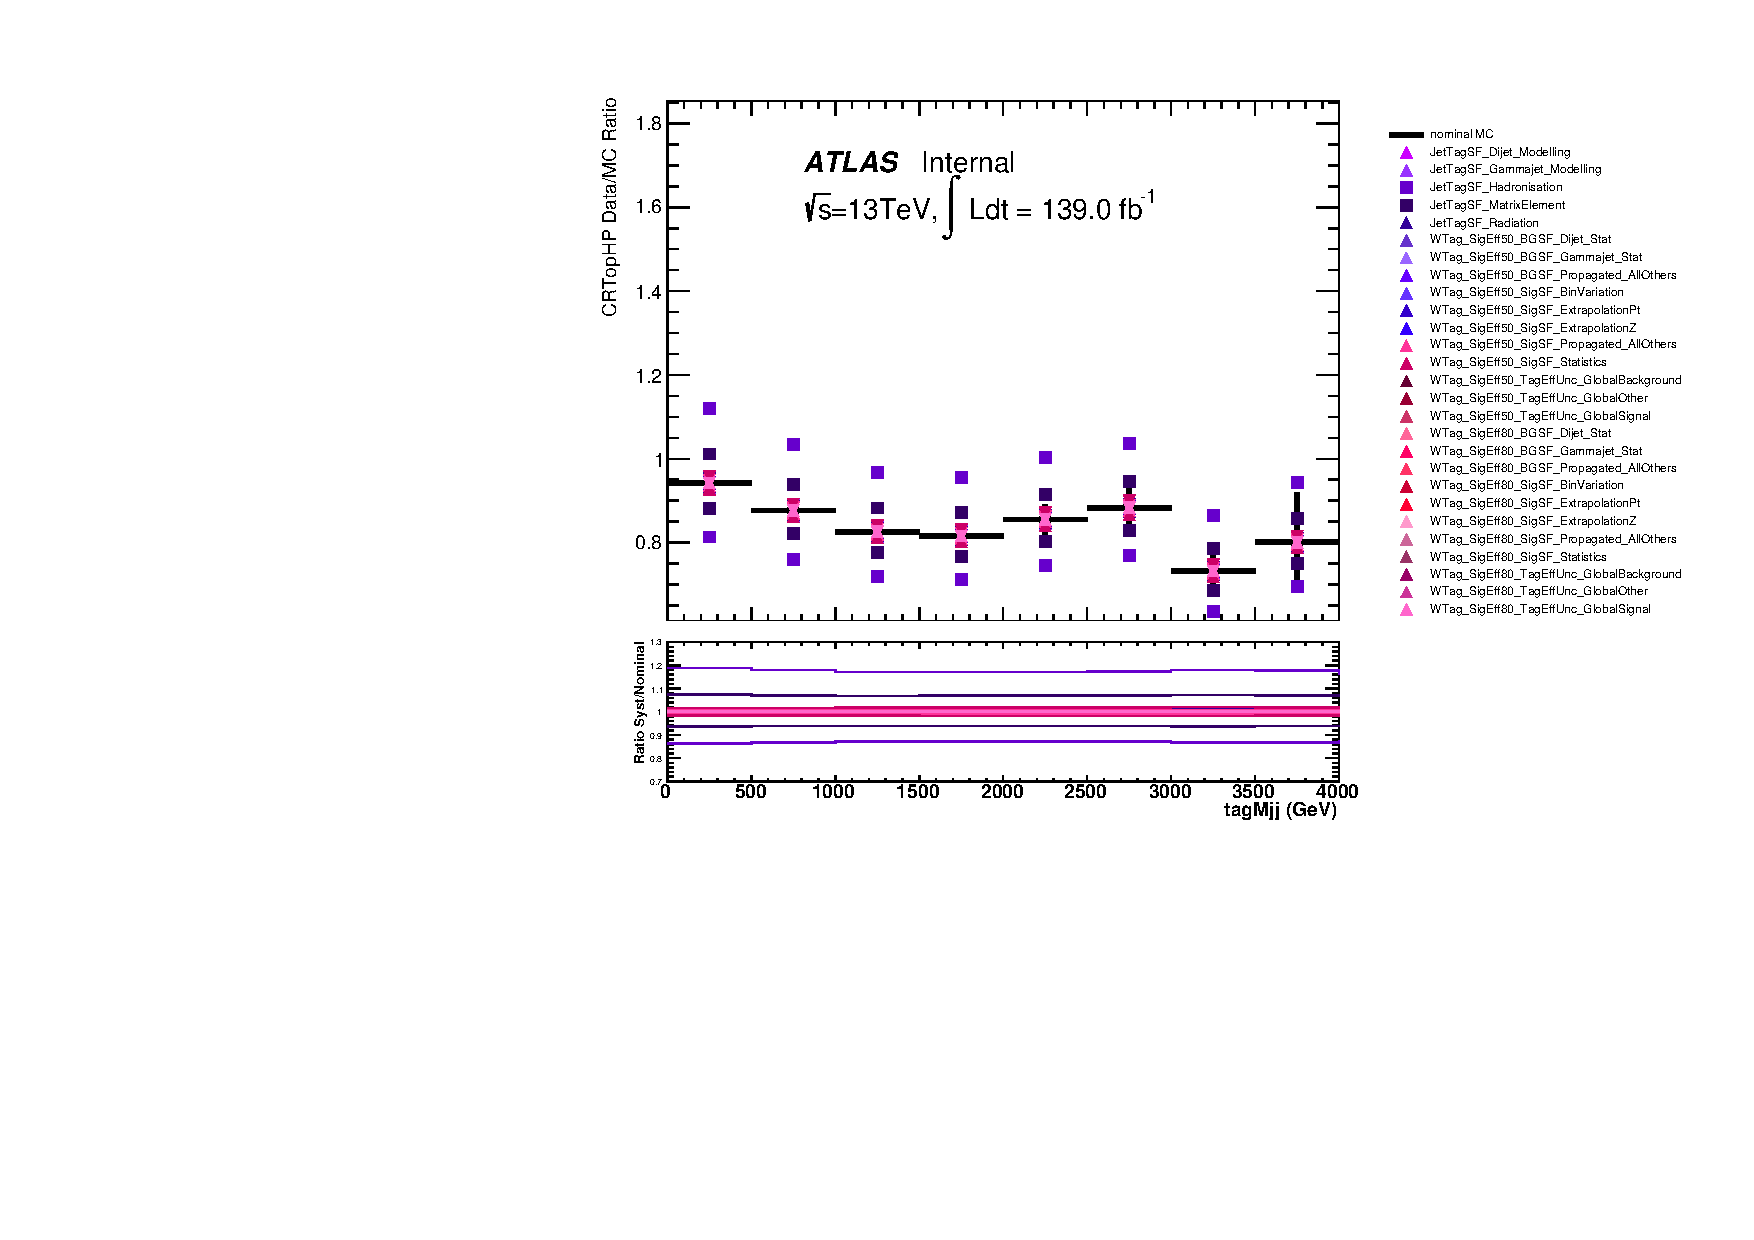
\includegraphics[width=\textwidth]{figures/1lep/VTaggerUnc/VTagCRTopHPtagMjj_SystBreakDown.pdf}
        \caption{Merged HP TopCR}
        \label{fig:MergedHPTopCR}
    \end{subfigure}
%    \hfill % This adds a bit of horizontal spacing between figures
    \begin{subfigure}[b]{0.3\textwidth}
        \centering
        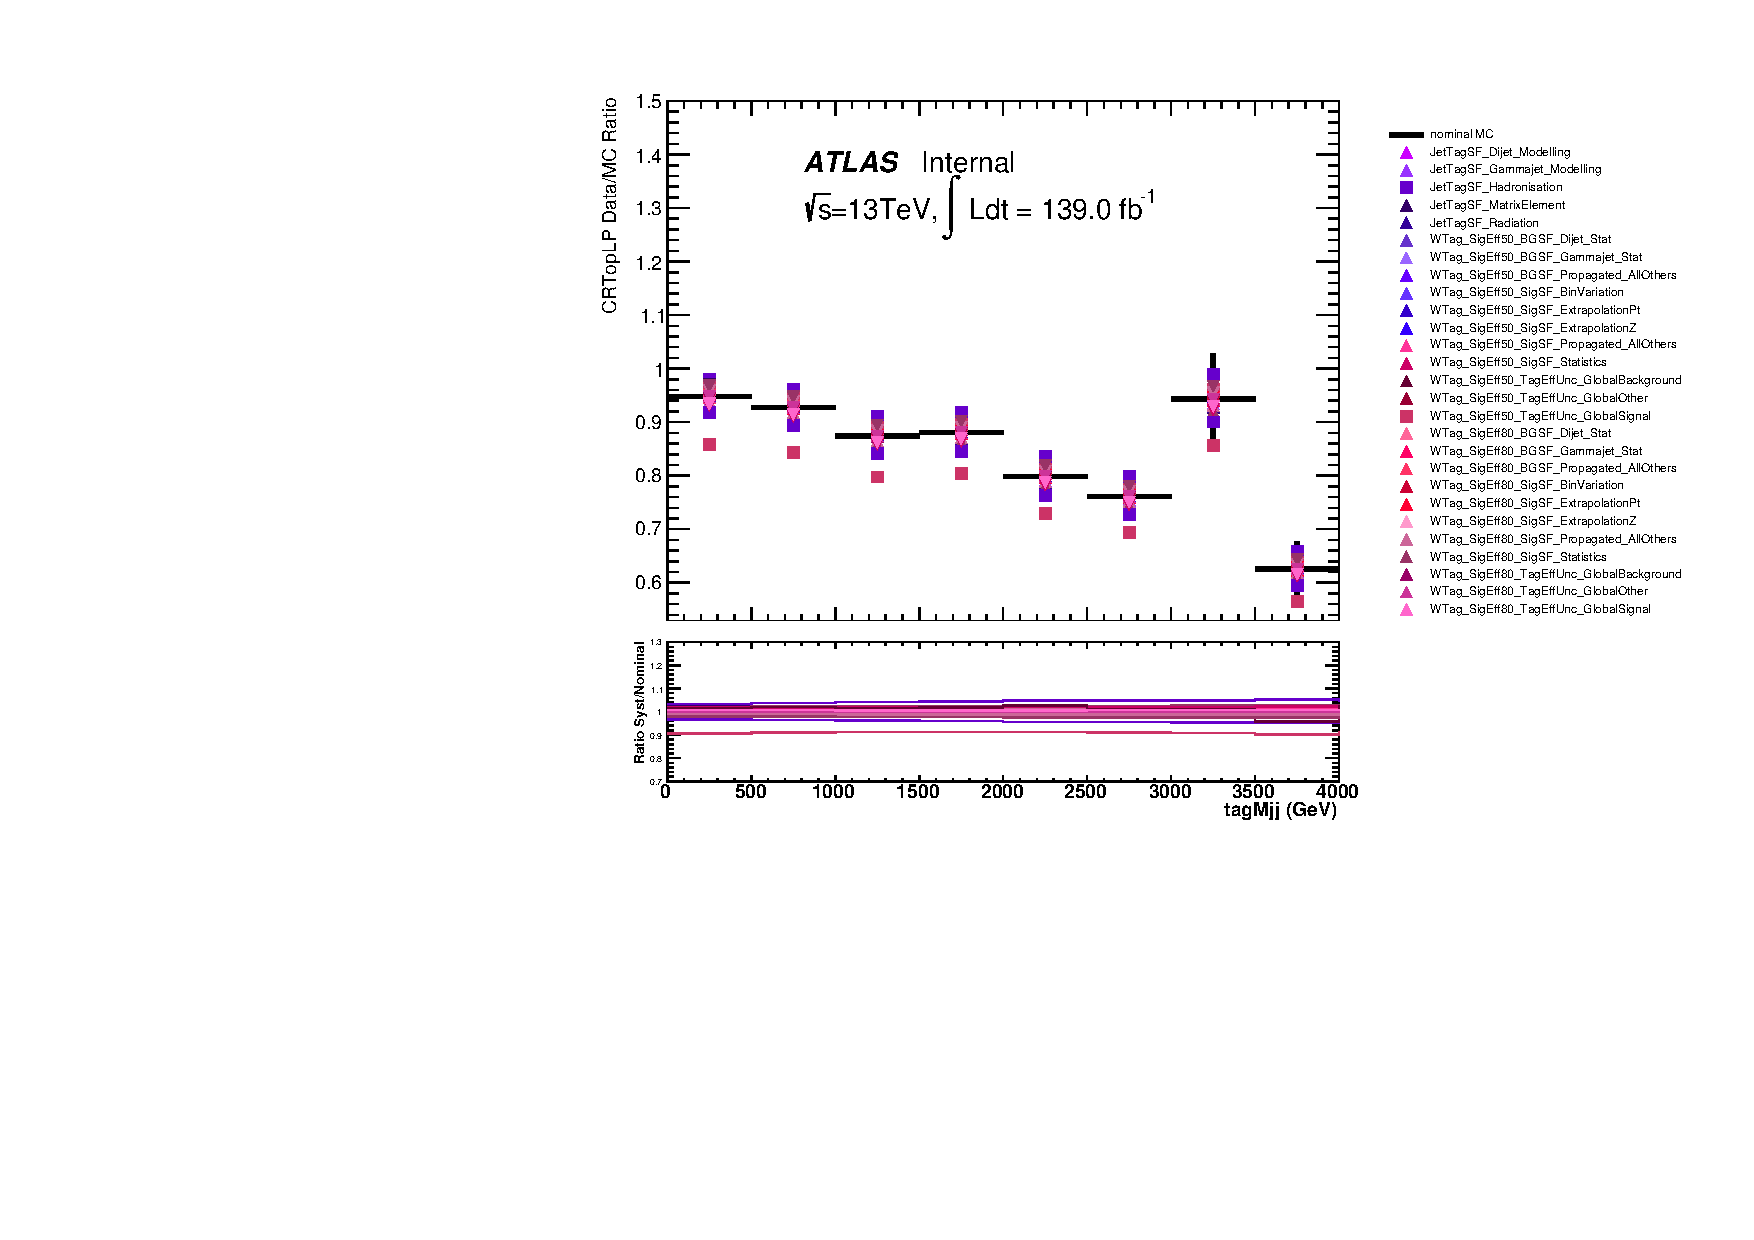
\includegraphics[width=\textwidth]{figures/1lep/VTaggerUnc/VTagCRTopLPtagMjj_SystBreakDown.pdf}
        \caption{Merged LP TopCR}
        \label{fig:MergedLPTopCR}
    \end{subfigure}
%    \hfill % This adds a bit of horizontal spacing between figures
    \begin{subfigure}[b]{0.3\textwidth}
        \centering
        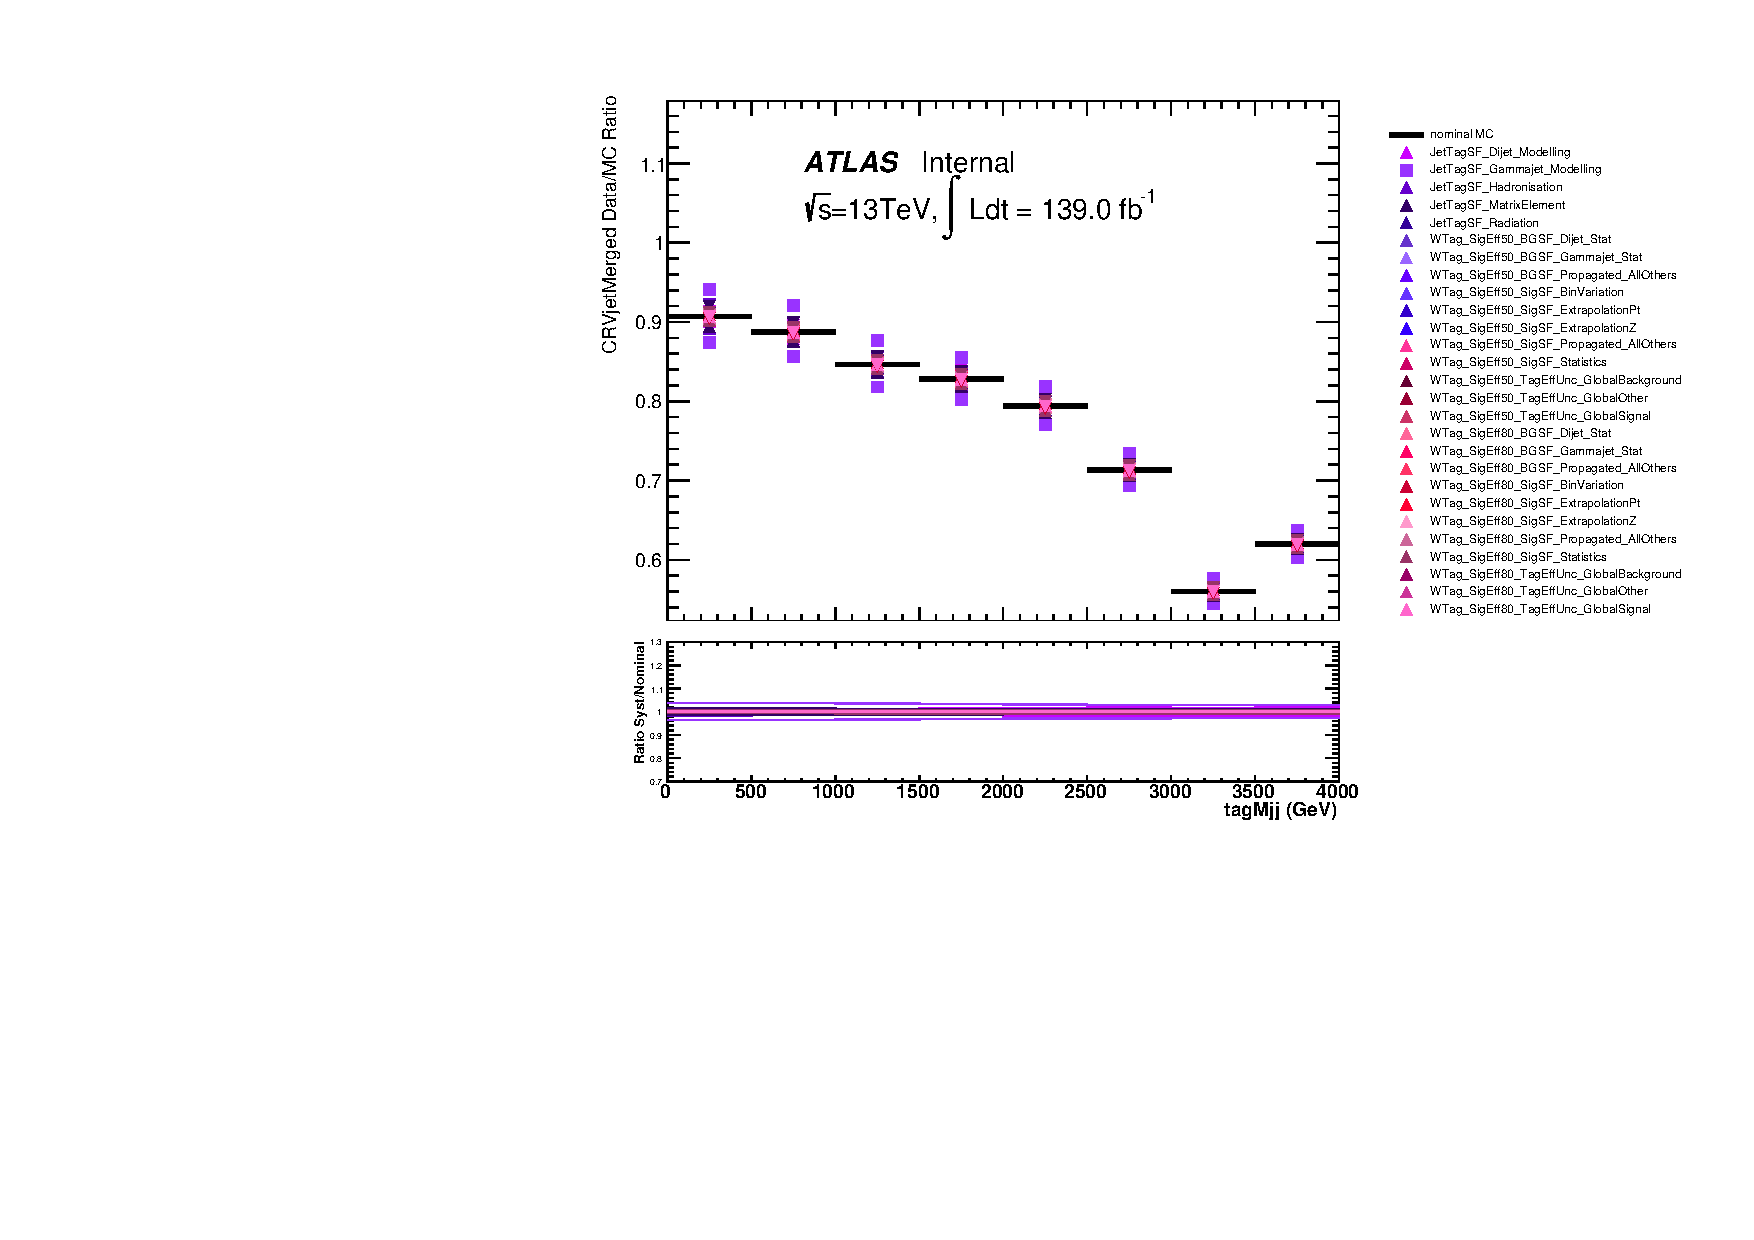
\includegraphics[width=\textwidth]{figures/1lep/VTaggerUnc/VTagCRVjetMergedtagMjj_SystBreakDown.pdf}
        \caption{Merged Wjets CR}
        \label{fig:MergedWjetsCR}
    \end{subfigure}
    \caption{Comparison of boson tagging scale factors in the 1-lepton channel.}
    \label{fig:1LepVTaggerUnc}
\end{figure}


%%%\begin{figure}[ht]
%%%    \centering
%%%        \subfigure[Merged CR]{\includegraphics[width=0.3\textwidth]{figures/2lep/taggerSF/0_MTagMerJets_SYS_CRVjet.pdf}}
%%%    	\subfigure[Merged HP SR]{\includegraphics[width=0.3\textwidth]{figures/2lep/taggerSF/0_MTagMerJets_SYS_SRVBS_HP.pdf}}
%%%        \subfigure[Merged LP SR]{\includegraphics[width=0.3\textwidth]{figures/2lep/taggerSF/0_MTagMerJets_SYS_SRVBS_LP.pdf}}
%%%        \caption{ Data/MC ratios as a function of the mass of the tagging jets in the 2-lepton channel. All tagger SF related uncertainties are plotted. The plots are before applying the re-weighting described in \ref{subsec:mjj_reweight_2lep}. All bins containing more than 5\% of signal are blinded in the SRs. } 
%%%    \label{fig:2lep_bkgUnc_BT}
%%%\end{figure}


%%%\begin{figure}[ht]
%%%    \centering
%%%        \subfigure[Merged HP TopCR]{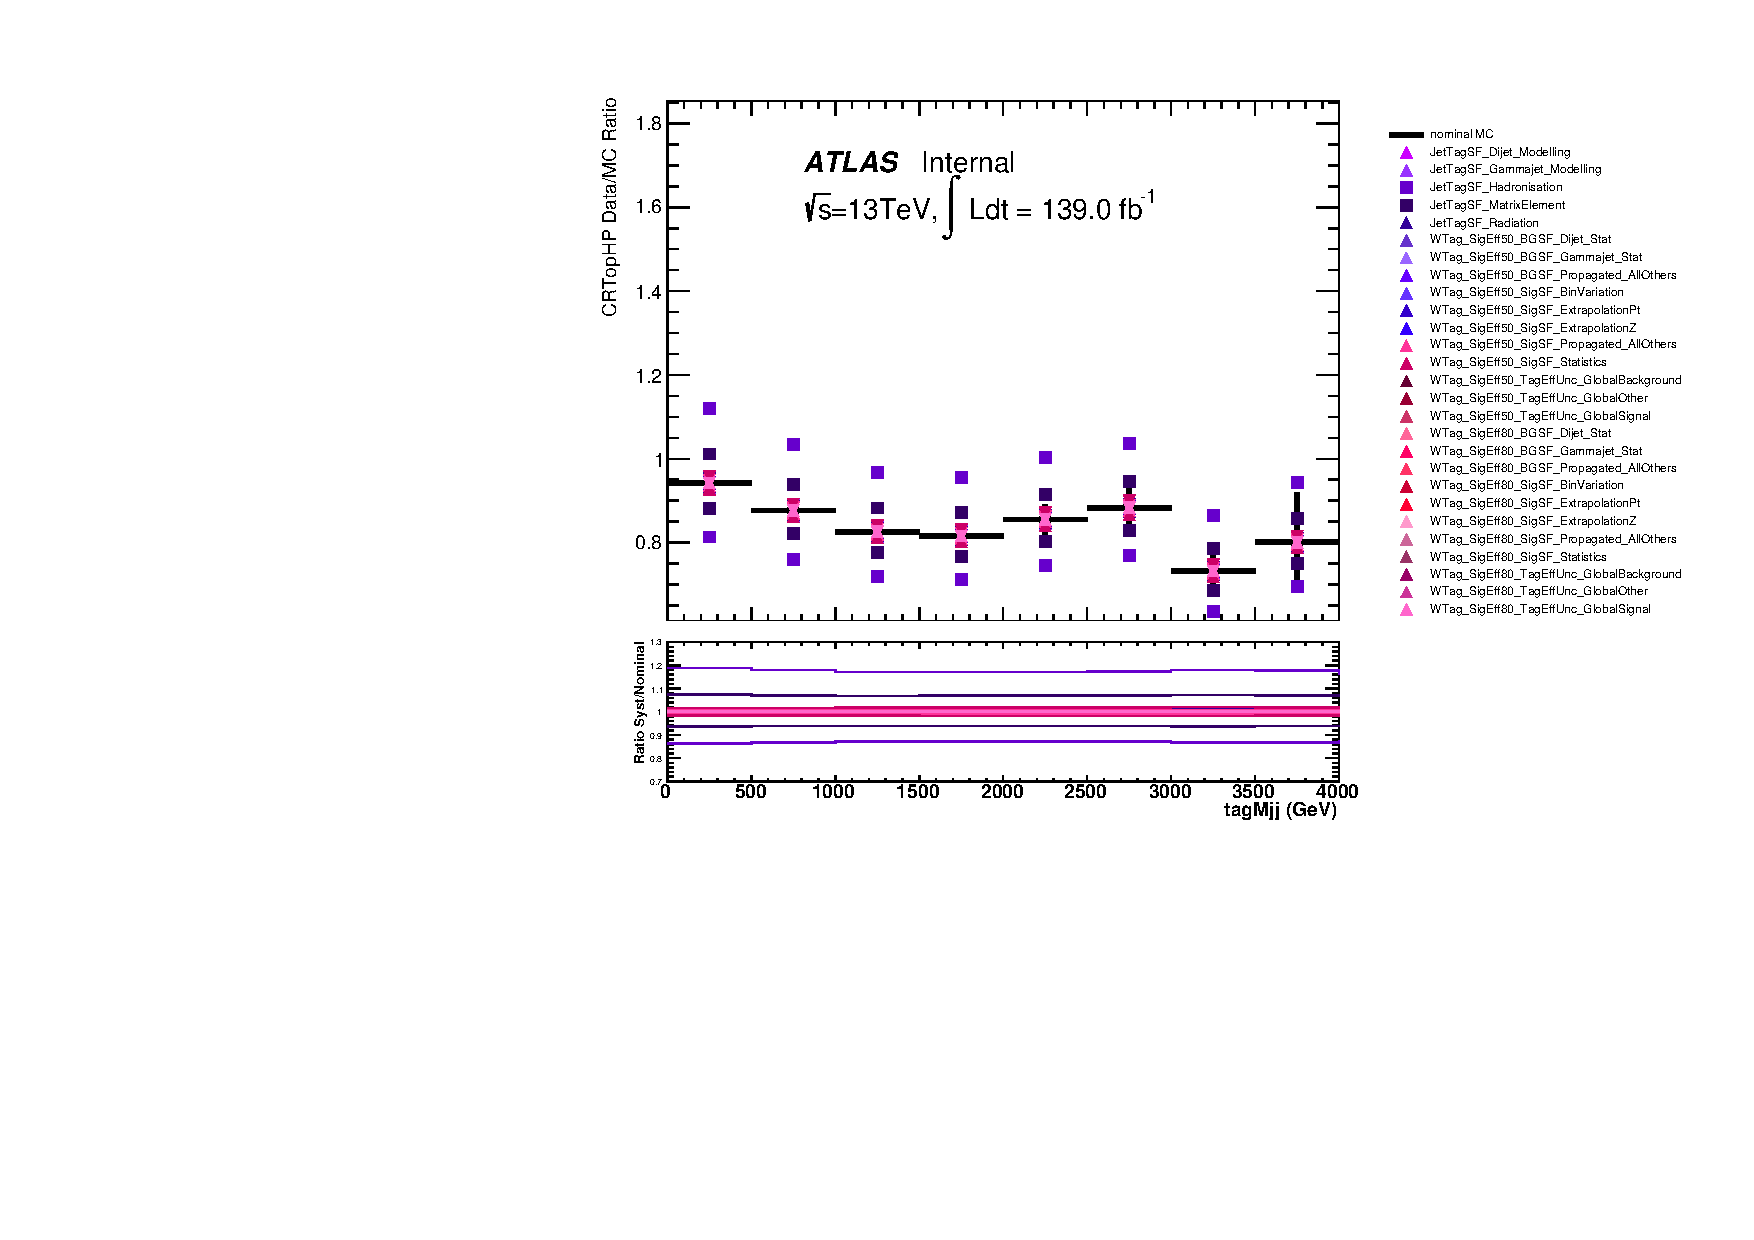
\includegraphics[width=0.3\textwidth]{figures/1lep/VTaggerUnc/VTagCRTopHPtagMjj_SystBreakDown.pdf}}
%%%    	\subfigure[Merged LP TopCR]{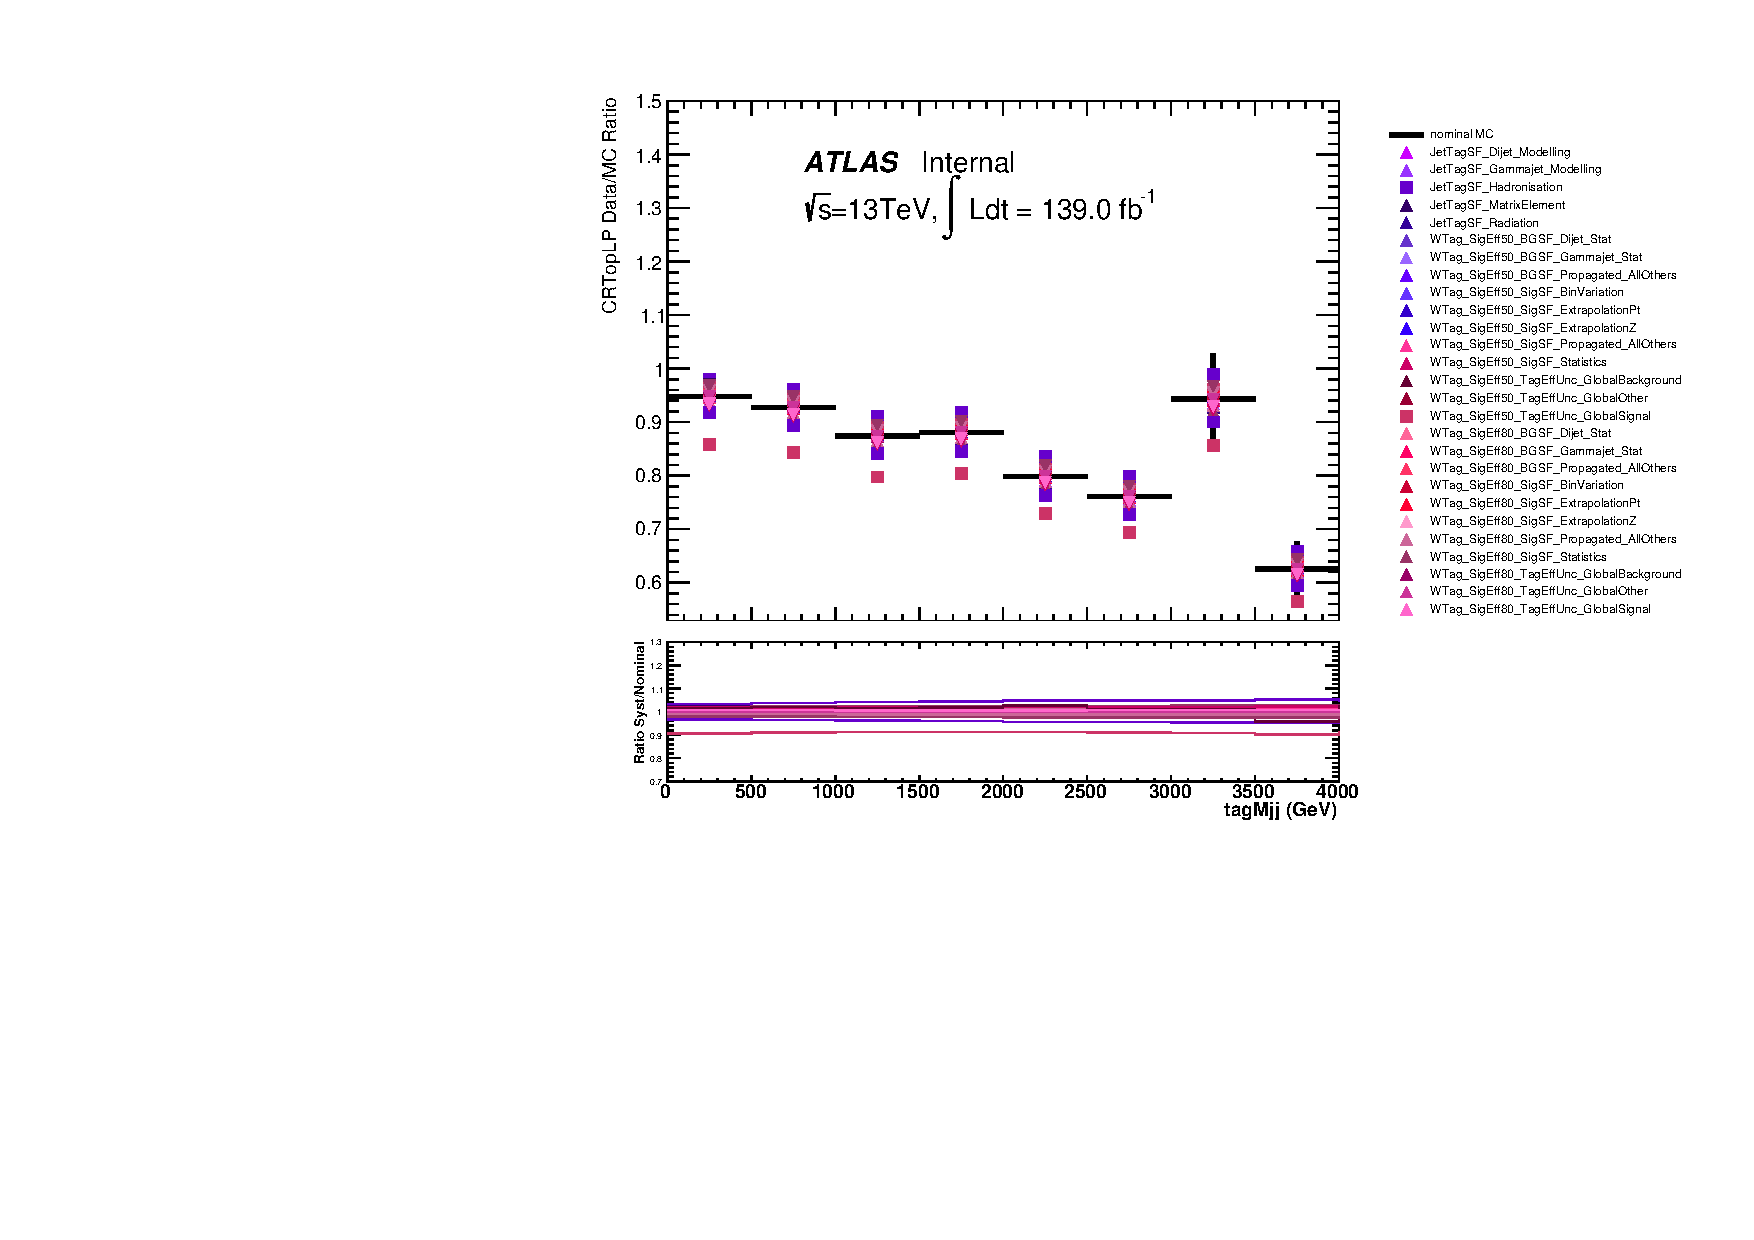
\includegraphics[width=0.3\textwidth]{figures/1lep/VTaggerUnc/VTagCRTopLPtagMjj_SystBreakDown.pdf}} 
%%%	\subfigure[Merged Wjets CR]{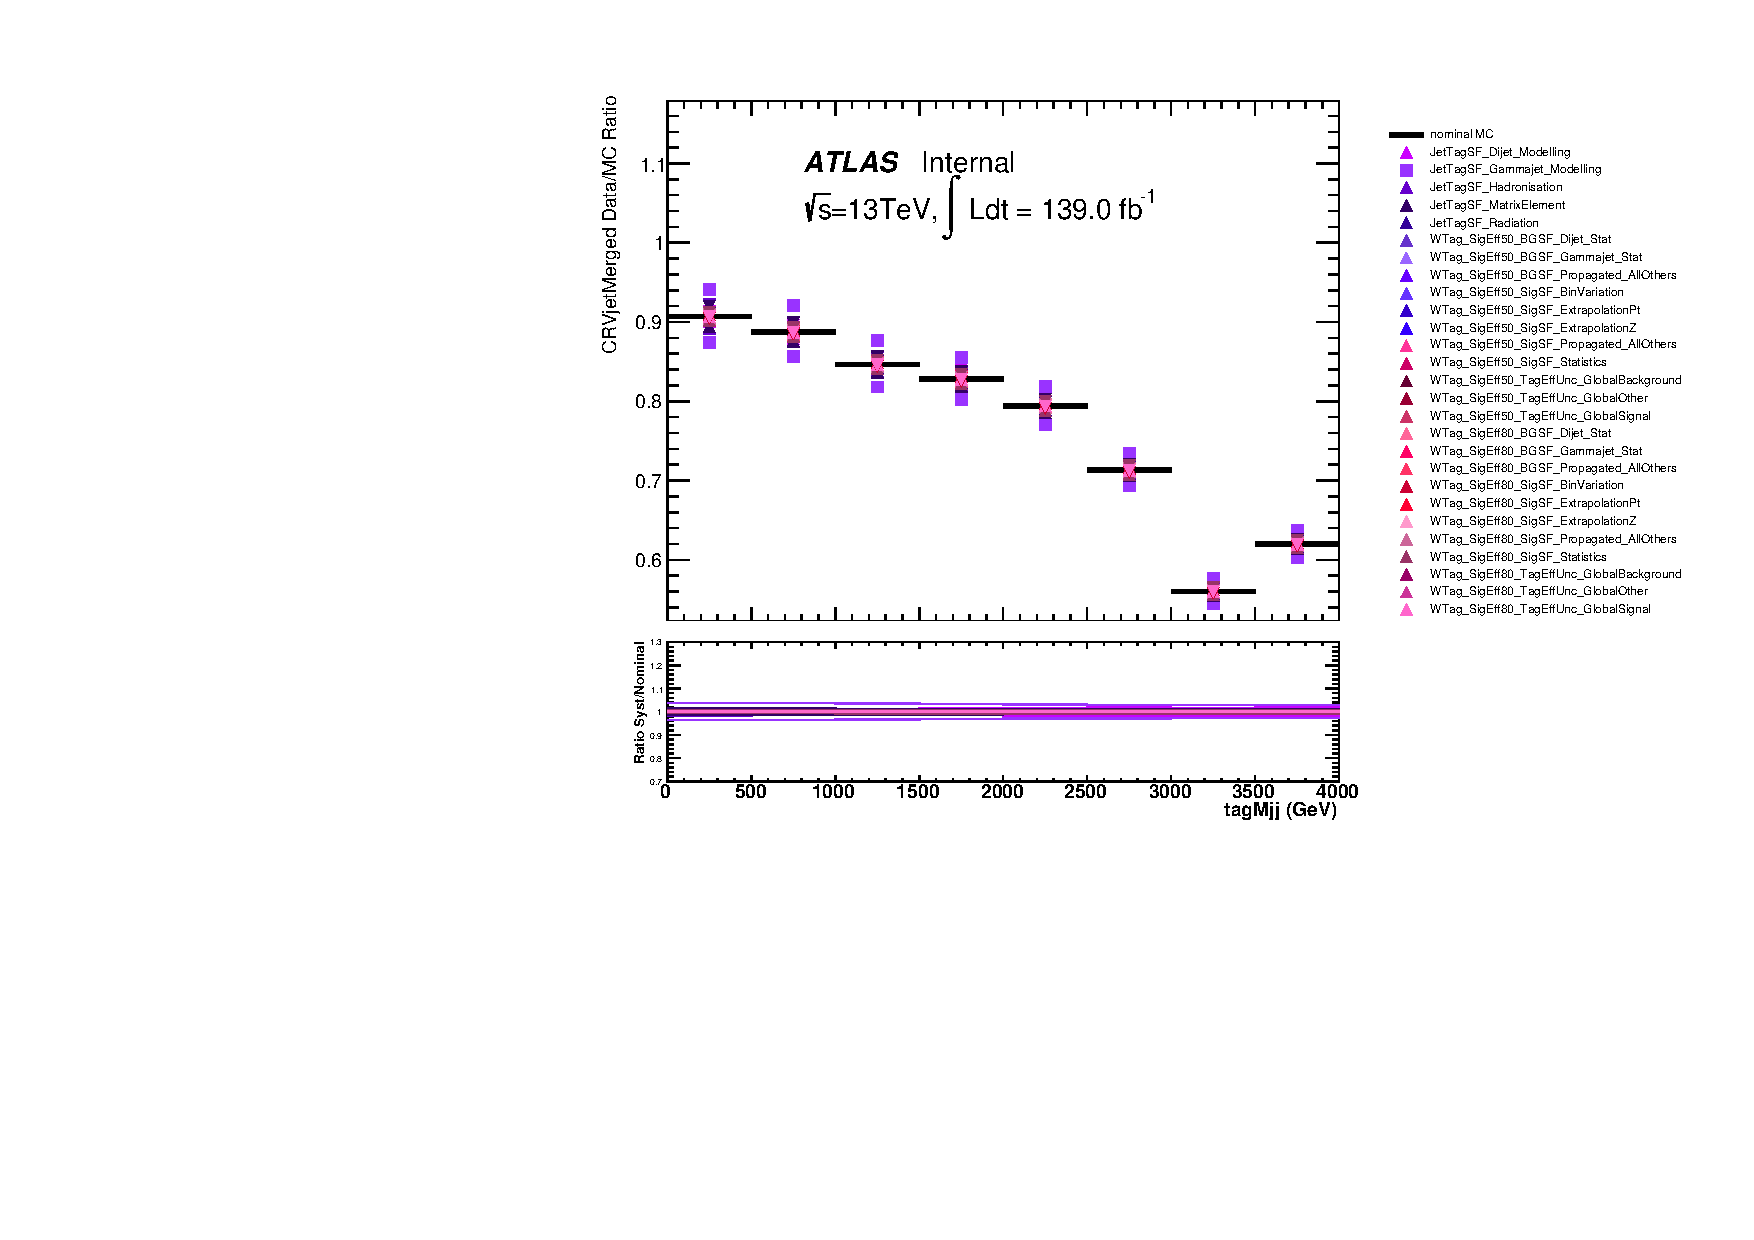
\includegraphics[width=0.3\textwidth]{figures/1lep/VTaggerUnc/VTagCRVjetMergedtagMjj_SystBreakDown.pdf}}
%%%        \caption{Comparison of boson tagging scale factors in the 1-lepton channel. } 
%%%    \label{fig:1LepVTaggerUnc}
%%%\end{figure}


%%%\begin{figure}[ht]
%%%    \centering
%%%      	\subfigure[signal: Merged CR]{\includegraphics[width=0.3\textwidth]{figures/0lep/systematics/systs/merged/plots/systvtagSigsig_RNN_CRVjet_Mer.pdf}}
%%%    	\subfigure[signal: Merged HP SR]{\includegraphics[width=0.3\textwidth]{figures/0lep/systematics/systs/merged/plots/systvtagSigsig_RNN_SRVBS_HP.pdf}}
%%%        \subfigure[signal: Merged LP SR]{\includegraphics[width=0.3\textwidth]{figures/0lep/systematics/systs/merged/plots/systvtagSigsig_RNN_SRVBS_LP.pdf}}\\
%%%      	\subfigure[background: Merged CR]{\includegraphics[width=0.3\textwidth]{figures/0lep/systematics/systs/merged/plots/systvtagBkgWjets_nom_Zjets_nom_diboson_stop_ttbar_nom_RNN_CRVjet_Mer.pdf}}
%%%    	\subfigure[background: Merged HP SR]{\includegraphics[width=0.3\textwidth]{figures/0lep/systematics/systs/merged/plots/systvtagBkgWjets_nom_Zjets_nom_diboson_stop_ttbar_nom_RNN_SRVBS_HP.pdf}}
%%%        \subfigure[background: Merged LP SR]{\includegraphics[width=0.3\textwidth]{figures/0lep/systematics/systs/merged/plots/systvtagBkgWjets_nom_Zjets_nom_diboson_stop_ttbar_nom_RNN_SRVBS_HP.pdf}}\\
%%%        \caption{Effect of all tagger SF related uncertainties in the 0-lepton channel on the signal MC and on all background MCs together.} 
%%%    \label{fig:0LepVTaggerUnc}
%%%\end{figure}

